\section{Stream computations}\label{sec:streams}

The core notion of our theory of IVM is the \textbf{stream}.  In this
section we introduce streams as infinite sequences of values, and
define computations on streams.

\subsection{Streams and stream operators}\label{sec:notation}

$\N$ is the set of natural numbers (from 0), $\B$ is the set of
Booleans, $\Z$ is the set of integers, and $\R$ is the set of real
numbers.

\begin{definition}[stream]
Given a set $A$, a \defined{stream} \emph{of values from $A$}, or an
\emph{$A$-stream}, is a function $\N \rightarrow A$.  $\stream{A}
\defn \{ s \,|\, s : \N \to A \}$ is the set of all $A$-streams.
\end{definition}

When $s\in\stream{A}$ and $t\in\N$ we
write $s[t]$ for the $t$-th element of the stream $s$.

\begin{definition}[stream operator]
A \defined{stream operator} is a function
$T:\stream{A_0}\times\cdots\times\stream{A_{n-1}}\to\stream{B}$.
\end{definition}

\begin{definition}(lifting)
Given a (scalar) function $f: A \to B$,
we define a stream operator $\lift{f} :\stream{A} \to \stream{B}$
by \emph{lifting} the function $f$ pointwise in time: $(\lift{f})(s) \defn f \circ s$.
Equivalently, $((\lift{f})(s))[t] \defn f(s[t])$.
This extends to functions of multiple arguments.
\end{definition}

\ifstreamexamples
For example, $(\lift{(\lambda x.(2x))})(id) = \sv{0 2 4 6 8}$.
\fi

\begin{proposition}[distributivity]\label{prop:distributivity}
Lifting distributes over function composition:
$\lift{(f \circ g)} = (\lift{f}) \circ (\lift{g})$.
\end{proposition}
\begin{comment}
\begin{proof}
This is easily proved by using associativity of function composition:
$\forall s~.~(\lift{(f \circ g)})(s) = (f \circ g) \circ s =
f \circ (g \circ s) = f \circ (\lift{g})(s) = (\lift{f})((\lift{g})(s)) =
(\lift{f} \circ \lift{g})(s).$
\end{proof}
\end{comment}

We say that two \dbsp programs are \defined{equivalent} if they compute the same
input-output function on streams.
We use the symbol $\cong$ to indicate that two circuits are
equivalent.  For example, Proposition~\ref{prop:distributivity}
states the following circuit equivalence:

\noindent
\begin{tabular}{m{3.5cm}m{.3cm}m{3.5cm}}
\begin{tikzpicture}[auto,>=latex]
  \node[] (input) {$s$};
  \node[block, right of=input] (g) {$\lift{g}$};
  \node[block, right of=g] (f) {$\lift{f}$};
  \node[right of=f] (output) {$o$};
  \draw[->>] (input) -- (g);
  \draw[->>] (g) -- (f);
  \draw[->>] (f) -- (output);
\end{tikzpicture}
&
$\cong$
&
\begin{tikzpicture}[auto,>=latex]
    \node[] (input) {$s$};
    \node[block, right of=input, node distance=1.5cm] (fg) {$\lift{(f \circ g)}$};
    \node[right of=fg, node distance=1.5cm] (output) {$o$};
    \draw[->>] (input) -- (fg);
    \draw[->>] (fg) -- (output);
\end{tikzpicture}
\end{tabular}

\subsection{Streams over abelian groups}\label{sec:abelian}

For the rest of the technical development we require the set of values
$A$ of a stream $\stream{A}$ to form a commutative group $(A, +, 0_A,
-)$.  The \emph{plus} defines what it means to add new data, while the
\emph{minus} allows us to compute differences (deltas).  We show later
that this restriction is not a problem for using \dbsp with relational
data.

\subsubsection{Delays and time-invariance}\label{sec:delay}

\begin{definition}[Delay]
The \defined{delay operator}\footnote{The name $\zm$ comes from the
DSP literature, and is related to the
z-transform~\cite{rabiner-book75}.}  $\zm$ produces an output stream
by delaying its input by one step: $\zm_A: \stream{A} \to \stream{A}$:
%\begin{tabular}{m{5cm}m{3cm}}
$$
\zm_A(s)[t] \defn   \begin{cases}
0_A      & \text{when}~t=0 \\
s[t - 1] & \text{when}~t\geq1
\end{cases}
$$
%&
%\begin{tikzpicture}[auto,node distance=1cm,>=latex]
%    \node[] (input) {$s$};
%    \node[block, right of=input] (z) {$\zm$};
%    \node[right of=z] (output) {$o$};
%    \draw[->] (input) -- (z);
%    \draw[->] (z) -- (output);
%\end{tikzpicture}
%\end{tabular}
\end{definition}

We often omit the type parameter $A$, and write just $\zm$.
\ifstreamexamples
For example, $\zm(\id) = \sv{0 0 1 2 3}$.
\fi

\begin{definition}[Time invariance]
A stream operator $S: \stream{A} \to \stream{B}$ is \defined{time-invariant} (TI) if
$S(\zm_A(s)) = \zm_B(S(s))$ for all $s \in \stream{A}$; in other words, if
the following two circuits are equivalent:
\end{definition}

\begin{tabular}{m{3cm}m{.5cm}m{3cm}}
\begin{tikzpicture}[auto,>=latex]
  \node[] (input) {$s$};
  \node[block, right of=input] (S) {$S$};
  \node[block, right of=S] (z) {$\zm$};
  \node[right of=z] (output) {$o$};
  \draw[->>] (input) -- (S);
  \draw[->>] (S) -- (z);
  \draw[->>] (z) -- (output);
\end{tikzpicture}
&
$\cong$
&
\begin{tikzpicture}[auto,>=latex]
  \node[] (input) {$s$};
  \node[block, right of=input] (z) {$\zm$};
  \node[block, right of=z] (S) {$S$};
  \node[right of=S] (output) {$o$};
  \draw[->>] (input) -- (z);
  \draw[->>] (z) -- (S);
  \draw[->>] (S) -- (output);
\end{tikzpicture}
\end{tabular}

The output of a TI operator only depends on its input, but never on
the ``logical clock'' value.  For example the operator $S(s)[t] = s[t]
+ t$ is \emph{not} TI.  The composition of TI operators of any number
of inputs is TI. The delay operator $\zm$ is TI.  \dbsp only uses TI
operators.

%\begin{definition}
%We say that a function between groups $f: A \to B$ has the \emph{zero-preservation
%property} if $f(0_A) = 0_B$.  We write $\zpp{f}$.
%\end{definition}
%
%A lifted operator $\lift{f}$ is TI iff $\zpp{f}$.

\subsubsection{Causal and strict operators}\label{sec:causal}

The definitions in this section are used to argue that some circuits
with cycles are well-defined.

\begin{definition}[Causality]
A stream operator \\ $S:\stream{A}\to\stream{B}$
is \defined{causal} when $\forall s,s'\in\stream{A}$,
and $\forall t \in \N$ we have:
$
(\forall i \leq t~.~s[i]=s'[i]) \Rightarrow S(s)[t]=S(s')[t].
$
\end{definition}

\noindent
In other words, the output value at time $t$ can only depend on input
values from times $t' \leq t$ (they cannot ``look'' into the future).
Operators produced by lifting are causal, and $\zm$ is causal.  The
composition of causal operators is causal.  \dbsp only uses causal
operators.

\begin{definition}[Strictness]
A stream operator \\ $F:\stream{A}\to\stream{B}$
is \defined{strict}
if  $\forall s,s'\in\stream{A}, \forall t \in \N$ we have:
$(\forall i<t~.~s[i]=s'[i]) \Rightarrow F(s)[t]=F(s')[t].$
\end{definition}

In other words, the $t$-th output of $F(s)$ can depend only on
``past'' values of the input $s$, between $0$ and $t-1$.  In
particular, $F(s)[0] = 0_B$ is the same for all $s \in \stream{A}$.
Strict operators are causal, but in addition, the current output can
only depend on previous inputs.  Lifted operators in general are
\emph{not} strict.  $\zm$ is strict.  Strict operators can compute
their $k$-th output before having received their corresponding input.

\begin{proposition}
\label{prop-unique-fix}
For a strict $F: \stream{A} \to \stream{A}$ the equation ~$\alpha=F(\alpha)$~ has a unique
solution $\alpha \in \stream{A}$, denoted by $\fix{\alpha}{F(\alpha)}$.
\end{proposition}

Thus every strict operator from a set to itself has a unique fixed
point.  The simple proof relies on strong induction, showing that the
solution $\alpha[t]$ depends only on the values of $\alpha$ prior to
$t$.

Consider a circuit with a strict ``feedback'' edge $F$:
\begin{center}
\begin{tikzpicture}[>=latex]
    \node[] (input) {$s$};
    \node[block, right of=input] (f) {$T$};
    \node[right of=f, node distance=1.2cm] (output) {$\alpha$};
    \node[block, below of=f, node distance=.6cm] (z) {$F$};
    \draw[->>] (input) -- (f);
    \draw[->>] (f) -- node (mid) {} (output);
    \draw[->>] (mid.center) |-  (z);
    \draw[->>] (z.west) -- ++(-.4,0) |- ([yshift=1mm]f.south west);
\end{tikzpicture}
\end{center}

This circuit is a well-defined function on streams, because the $F$
operator can produce an output before having received the
corresponding input, enabling $T$ to compute the first output
immediately.

%\begin{lemma}
%\label{lemma-causal-strict}
%If $F: \stream{B} \to \stream{B}$ is strict and $T: \stream{A} \times \stream{B} \to \stream{B}$ is causal, then for fixed $s$ the operator
%$\lambda\alpha.T(s,F(\alpha)): \stream{A} \to \stream{B}$ is strict.
%\end{lemma}

\begin{lemma}\label{feedback-semantics}
\label{cor-loop}
If $F: \stream{B} \to \stream{B}$ is strict and $T: \stream{A} \times \stream{B} \to \stream{B}$ is causal,
the operator $Q(s)=\fix{\alpha}{T(s,F(\alpha))}$ is well-defined and causal.
If, moreover, $F$ and $T$ are TI then so is $Q$.
\end{lemma}

Most \dbsp computations are built using just lifted functions and
delays.  We add two more operators in \secref{sec:nested} to support
recursive functions.

\subsection{Integration and differentiation}\label{sec:abelianstreams}

Remember that we require the elements of a stream to come from an abelian group $A$.
Streams themselves form an abelian group:

\begin{proposition}
The structure $(\stream{A},+,0,-)$, obtained by lifting the $+$ and unary $-$ operations of $A$,
is an abelian group.  0 is the stream with all values $0_A$.
\end{proposition}

\noindent
To simplify the notation, we write $a + b$ for streams $a, b$ instead
of $a (\lift{+}) b$; we also write $-a$ instead of $(\lift{-})a$.
Stream addition and negation are causal, TI operators.

\begin{definition}
Given abelian groups $A$ and $B$ we call a stream operator
$S: \stream{A} \rightarrow \stream{B}$ \defined{linear} if it is a group homomorphism, that is,
$S(a+b)=S(a)+S(b)$ (and therefore $S(0)=0$ and $S(-a)=-S(a)$).
\end{definition}

We write LTI for ``linear and TI''.  Given a linear function $f: A \to
B$, the stream operator $\lift{f}$ is LTI.  $\zm$ is also LTI.

\begin{definition}(bilinear)
A function of two arguments $f: A \times B \to C$ where $A, B, C$ are
groups, is \emph{bilinear} if it is linear separately in each argument
(i.e., it distributes over addition): $\forall a, b, c, d~.~f(a+b, c)
= f(a, c) + f(b, c)$, and $f(a, c+d) = f(a, c) + f(c, d).$
\end{definition}

This definition extends to stream operators.
The lifting of a bilinear function $f$ is
a bilinear stream operator $\lift{f}$.  An example
is lifted multiplication:
$f: \stream{\N} \times \stream{\N} \to \stream{\N}, f(a, b)[t] = a[t]\cdot b[t]$.

%The composition of (bi)linear operators with linear operators
%is (bi)linear (since homomorphisms compose).

\begin{definition}[Differentiation]
The \defined{differentiation operator} $\D_{\stream{A}} : \stream{A}
\to \stream{A}$ is: $\D(s) \defn s - \zm(s)$.
\begin{center}
\begin{tikzpicture}[auto,>=latex,node distance=1cm]
    \node[] (input) {$s$};
    \node[block, shape=circle, right of=input, inner sep=0pt,node distance=2cm] (plus) {$+$};
    \node[right of=plus] (output) {$\D(s)$};
    \draw[->>] (input) -- node (i) {} (plus);
    \node[block, below of=i, node distance=.8cm] (z) {$\zm$};
    \node[block, shape=circle, right of=z, inner sep=0pt] (minus) {$-$};
    \draw[->>] (plus) -- (output);
    \draw[->>] (i) -- (z);
    \draw[->>] (z) -- (minus);
    \draw[->>] (minus) -- (plus);
\end{tikzpicture}
\end{center}
\end{definition}
We generally omit the type, and write just $\D$.
The value of $\D(s)[t] = s[t] - s[t-1]$ if $t > 0$.
If $s$ is a stream, then $\D(s)$ is the \emph{stream of changes} of $s$.

As an example:
{
\noindent \small
\begin{align*}
  \D(\sv{0 1 2 1 0}) &= \\
  \sv{0 1 2 1 0} - \zm(\sv{0 1 2 1 0}) &=\\
  \sv{0 1 2 1 0} - \sv{0 0 1 2 1} &= \sv{0 1 1 -1 -1}
%  &\sv{0-0 1-0 2-1 1-2 0-1} =\\
\end{align*}
}

\begin{proposition}
\label{prop-diff-properties}
$\D$ is causal and LTI.
\end{proposition}

The ``feedback loop'' built from linear operator and a delay is
linear:

\begin{proposition}
\label{prop-rec-linear}
Is $S$ is causal and LTI, the operator
$Q(s)=\fix{\alpha}{S(s+\zm(\alpha))}$ is well-defined and LTI:

\begin{center}
\begin{tikzpicture}[>=latex]
    \node[] (input) {$s$};
    \node[block, shape=circle, right of=input, inner sep=0pt, node distance=.8cm] (plus) {$+$};
    \node[block, right of=plus, node distance=.8cm] (Q) {$S$};
    \node[right of=Q, node distance=1.4cm] (output) {$\alpha$};
    \node[block, below of=Q, node distance=.6cm] (z) {$\zm$};
    \draw[->>] (input) -- (plus);
    \draw[->>] (plus) -- (Q);
    \draw[->>] (Q) -- node (mid) {} (output);
    \draw[->>] (mid.center) |-  (z);
    \draw[->>] (z) -| (plus);
\end{tikzpicture}
\end{center}
\end{proposition}

The integration operator ``reconstitutes'' a stream from its changes:

\begin{definition}[Integration]
The \defined{integration operator} $\I_{\stream{A}} : \stream{A} \to
\stream{A}$ is $\I(s) \defn \lambda s . \fix{\alpha}{(s +
  \zm(\alpha))}$:
\begin{center}
\begin{tikzpicture}[auto,>=latex, node distance=1.1cm]
    \node[] (input) {s};
    \node[block, shape=circle, right of=input, inner sep=0pt] (plus) {$+$};
    \node[right of=plus, node distance=1.9cm] (output) {$\I(s) = o$};
    \node[block, below of=plus, node distance=.8cm] (z) {$z^{-1}$};
    \draw[->>] (input) -- (plus);
    \draw[->>] (plus) -- node (o) {} (output);
    \draw[->>] (o) |- (z);
    \draw[->>] (z) -- (plus);
\end{tikzpicture}
\end{center}
\end{definition}

\noindent
We also omit the type, and write just $\I$.  This is the circuit from
Proposition~\ref{prop-rec-linear} using the identity for $S$.

\begin{proposition}
$\I(s)$ is the discrete (indefinite) integral applied to the stream $s$:
$\I(s)[t] = \sum_{i \leq t} s[i]$.
\end{proposition}
\begin{proof}
Using the notation $o = \I(s)$ to make formulas more readable, we can
see the contents of stream $o$ is produced step by step.  Here are the
first three steps:
\begin{align*}
  o[0] &= s[0] + (\zm(o))[0] = s[0] + 0 = s[0] \\
  o[1] &= s[1] + (\zm(o))[1] = s[1] + o[0] = s[1] + s[0] \\
  o[2] &= s[2] + (\zm(o))[2] = s[2] + o[1] = s[2] + (s[1] + s[0])
\end{align*}
\end{proof}

\begin{proposition}
\label{prop-integ-properties}
$\I$ is causal and LTI.
\end{proposition}

\begin{theorem}[Inversion]
\label{inverses}
$\I$ and $\D$ are inverses of each other: $\forall s~.~\I(\D(s)) =
\D(\I(s)) = s$.
\end{theorem}

\noindent
\begin{tabular}{m{2.5cm}m{.2cm}m{.8cm}m{.2cm}m{2.5cm}}
\begin{tikzpicture}[auto,>=latex, node distance=.85cm]
    \node[] (input) {$s$};
    \node[block, right of=input] (I) {$\I$};
    \node[block, right of=I] (D) {$\D$};
    \node[right of=D] (output) {$o$};
    \draw[->>] (input) -- (I);
    \draw[->>] (I) -- (D);
    \draw[->>] (D) -- (output);
\end{tikzpicture}
     & $\cong$ &
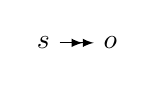
\begin{tikzpicture}[auto,>=latex, node distance=.85cm]
    \node[] (input) {$s$};
    \node[right of=input] (output) {$o$};
    \draw[->>] (input) -- (output);
\end{tikzpicture}
     & $\cong$ &
\begin{tikzpicture}[auto,>=latex, node distance=.85cm]
    \node[] (input) {$s$};
    \node[block, right of=input] (D) {$\D$};
    \node[block, right of=D] (I) {$\I$};
    \node[right of=I] (output) {$o$};
    \draw[->>] (input) -- (D);
    \draw[->>] (D) -- (I);
    \draw[->>] (I) -- (output);
\end{tikzpicture}
\end{tabular}

\section{Incremental view maintenance}\label{sec:incremental}

Here we define IVM and analyze its properties.

\begin{definition}
Given a unary stream operator $Q: \stream{A} \to \stream{B}$ we define the
\defined{incremental version} of $Q$ as:
\begin{equation}\label{def:inc}
\inc{Q} \defn \D \circ Q \circ \I.
\end{equation}
$\inc{Q}$ has the same ``type'' as $Q$: $\inc{Q}: \stream{A} \to \stream{B}$.
For an operator with multiple inputs we define
the incremental version by applying $\I$ to each input independently:
e.g., if $T: \stream{A} \times \stream{B} \rightarrow \stream{C}$ then
$\inc{T}(a, b) \defn \D (T(\I(a), \I(b)))$.
\end{definition}

%The following diagram illustrates the intuition behind this
%definition:
\begin{center}
\begin{tikzpicture}[auto,>=latex]
    \node[] (input) {$\Delta s$};
    \node[block, right of=input] (I) {$\I$};
    \node[block, right of=I] (Q) {$Q$};
    \node[block, right of=Q] (D) {$\D$};
    \node[right of=D] (output) {$\Delta o$};
    \draw[->>] (input) -- (I);
    \draw[->>] (I) -- node (s) {$s$} (Q);
    \draw[->>] (Q) -- node (o) {$o$} (D);
    \draw[->>] (D) -- (output);
    \draw[decorate, decoration = {brace, raise=10pt}] (input) -- (output)
    node[pos=.5, above=13pt]{$\inc{Q}$};
\end{tikzpicture}
\end{center}
If $Q(s) = o$ is a streaming operator, then $\inc{Q}$ operates on
streams of changes: $\inc{Q}(\Delta s) = \Delta o$.

Notice that our definition of incremental computation is meaningful only for \emph{streaming}
computations; this is in contrast to classic definitions, e.g.~\cite{gupta-idb95} which
consider only one change.  Generalizing the definition to operate on streams gives us
additional power, especially when operating with recursive queries.

The following is one of our central results:

\begin{proposition}(Properties of the incremental version):
\label{prop-inc-properties}
\begin{description}[nosep, leftmargin=\parindent]
\item[inversion:] $Q\mapsto\inc{Q}$ is bijective; $Q\mapsto \I\circ
  Q\circ\D$ is its inverse
%\item[invariance:] $\inc{+} = +, \inc{(\zm)} = \zm, \inc{-} = -, \inc{\I}=\I, \inc{\D}=\D$
\item[push/pull:] \label{prop-part-commutation}
    $Q \circ \I = \I \circ \inc{Q}$; $\D\circ Q = \inc{Q}\circ\D$
\item[chain:] $\inc{(Q_1\circ Q_2)} = \inc{Q_1}\circ\inc{Q_2}$
\item[add:] $\inc{(Q_1 + Q_2)} = \inc{Q_1} + \inc{Q_2}$
\item[cycle:] $\inc{(\lambda s. \fix{\alpha}{T(s,\zm(\alpha)}))} = \lambda s. \fix{\alpha}{\inc{T}(s,\zm(\alpha)})$
\end{description}
\end{proposition}

Here is the proof of the \defined{chain rule}, which states that
$\inc{(Q_1 \circ Q_2)} = \inc{Q_1} \circ \inc{Q_2}$.

\begin{tabular}{cr}
\begin{tikzpicture}[auto,>=latex]
  \node[] (input) {$\Delta i$};
  \node[block, right of=input] (I) {$\I$};
  \node[block, right of=I] (Q1) {$Q_1$};
  \node[block, right of=Q1] (Q2) {$Q_2$};
  \node[block, right of=Q2] (D) {$\D$};
  \node[right of=D] (output)  {$\Delta o$};
  \draw[->>] (input) -- (I);
  \draw[->>] (I) -- (Q1);
  \draw[->>] (Q1) -- (Q2);
  \draw[->>] (Q2) -- (D);
  \draw[->>] (D) -- (output);
\end{tikzpicture} &
$\cong$ \\
\begin{tikzpicture}[>=latex, node distance=.9cm]
  \node[] (input) {$\Delta i$};
  \node[block, right of=input] (I1) {$\I$};
  \node[block, right of=I1] (Q1) {$Q_1$};
  \node[block, right of=Q1] (D1) {$\D$};
  \node[block, right of=D1] (I2) {$\I$};
  \node[block, right of=I2] (Q2) {$Q_2$};
  \node[block, right of=Q2] (D2) {$\D$};
  \node[right of=D2] (output)  {$\Delta o$};
  \draw[->>] (input) -- (I1);
  \draw[->>] (I1) -- (Q1);
  \draw[->>] (Q1) -- (D1);
  \draw[->>] (D1) -- (I2);
  \draw[->>] (I2) -- (Q2);
  \draw[->>] (Q2) -- (D2);
  \draw[->>] (D2) -- (output);
\end{tikzpicture} &
$\cong$ \\
\begin{tikzpicture}[>=latex, node distance=1.2cm]
  \node[] (input) {$\Delta i$};
  \node[block, right of=input] (Q1) {$\inc{Q_1}$};
  \node[block, right of=Q1] (Q2) {$\inc{Q_2}$};
  \node[right of=Q2] (output)  {$\Delta o$};
  \draw[->>] (input) -- (Q1);
  \draw[->>] (Q1) -- (Q2);
  \draw[->>] (Q2) -- (output);
\end{tikzpicture}
\end{tabular}

\noindent In other words, \textbf{to incrementalize a composite query you can incrementalize
each sub-query independently}.  This gives us a simple, syntax-directed, deterministic recipe
for computing the incremental version of an arbitrarily complex query.

The \defined{cycle rule} states that the following circuits are equivalent:

\noindent
\begin{tabular}{m{4.4cm}m{.2cm}m{3cm}}
\begin{tikzpicture}[>=latex]
    \node[] (input) {$\Delta s$};
    \node[block, right of=input] (I) {$\I$};
    \node[block, right of=I] (f) {$T$};
    \node[block, right of=f, node distance=1.4cm] (D) {$\D$};
    \node[right of=D] (output) {$\Delta o$};
    \node[block, below of=f, node distance=.6cm] (z) {$\zm$};
    \draw[->>] (input) -- (I);
    \draw[->>] (I) -- (f);
    \draw[->>] (f) -- node (mid) {} (D);
    \draw[->>] (mid.center) |-  (z);
    \draw[->>] (z.west) -- ++(-.3,0) |- ([yshift=1mm]f.south west);
    \draw[->>] (D) -- (output);
\end{tikzpicture} & $\cong$ &
\begin{tikzpicture}[>=latex]
    \node[] (input) {$\Delta s$};
    \node[block, right of=input] (f) {$\inc{T}$};
    \node[right of=f, node distance=1.3cm] (output) {$\Delta o$};
    \node[block, below of=f, node distance=.6cm] (z) {$\zm$};
    \draw[->>] (input) -- (f);
    \draw[->>] (f) -- node (mid) {} (output);
    \draw[->>] (mid.center) |-  (z);
    \draw[->>] (z.west) -- ++(-.3,0) |- ([yshift=1mm]f.south west);
\end{tikzpicture}
\end{tabular}

In other words, the incremental version of a feedback loop around a
query is just the feedback loop with the incremental query for its
body.  This result will be used to implement recursive queries
in~\refsec{sec:recursion}.

To execute incremental queries efficiently, we want to compute
directly on streams of changes, without integrating them.  The
following theorems show how this can be done for linear and bi-linear
operators:

\begin{theorem}[Linear]\label{linear}
If $Q$ is LTI, we have $\inc{Q}=Q$.
\end{theorem}

This implies that stream operators $+$, $-$, $\I$, $\D$, and $\zm$ are
identical to their incremental versions.

\begin{theorem}[Bilinear]\label{bilinear}
Using the infix notation: if $\times$ is bilinear TI, we have:
\begin{eqnarray*}
\inc{(\Delta a \times \Delta b)} = \\
(\Delta a \times \Delta b ~+~ \zm(\I(\Delta a)) \times
\Delta b ~+~ \Delta a \times \zm(\I(\Delta b)) = \\
\Delta a \times \Delta b + \zm(a) \times \Delta b + \Delta a \times \zm(b)
\end{eqnarray*}
In pictures: \\
\noindent
\begin{tabular}{m{3.3cm}m{0cm}m{4cm}}
\begin{tikzpicture}[auto,>=latex]
    \node[] (a) {$\Delta a$};
    \node[block, right of=a] (ai) {$\I$};
    \node[below of=a, node distance=.8cm] (midway) {};
    \node[below of=midway, node distance=.8cm] (b) {$\Delta b$};
    \node[block, right of=b] (bi) {$\I$};
    \node[block, right of=midway, node distance=1cm] (q) {$\times$};
    \node[block, right of=q] (D) {$\D$};
    \node[right of=D] (output) {$\Delta o$};
    \draw[->>] (a) -- (ai);
    \draw[->>] (b) -- (bi);
    \draw[->>] (ai) -- (q);
    \draw[->>] (bi) -- (q);
    \draw[->>] (q) -- (D);
    \draw[->>] (D) -- (output);
\end{tikzpicture} &
$\cong$ &
\begin{tikzpicture}[auto,>=latex]
  \node[] (input1) {$\Delta a$};
  \node[below of=input1, node distance=1.6cm] (input2) {$\Delta b$};
  \node[block, right of=input1, node distance=1cm] (I1) {$\I$};
  \node[block, below of=I1,node distance=.8cm] (ab) {$\times$};
  \node[block, right of=input2, node distance=1cm] (I2) {$\I$};
  \draw[->>] (input1) -- (I1);
  \draw[->>] (input2) -- (I2);
  \draw[->>] (input1) |- ([yshift=-1mm]ab.north west);
  \draw[->>] (input2) |- ([yshift=1mm]ab.south west);
  \node[block, right of=I1] (ZI1) {$\zm$};
  \node[block, right of=I2] (ZI2) {$\zm$};
  \draw[->>] (I1) -- (ZI1);
  \draw[->>] (I2) -- (ZI2);
  \node[block, right of=ZI1] (DI1) {$\times$};
  \node[block, right of=ZI2] (DI2) {$\times$};
  \draw[->>] (ZI1) -- (DI1);
  \draw[->>] (ZI2) -- (DI2);
  \node[block, circle, right of=ab, inner sep=0cm, node distance=2cm] (sum) {$+$};
  \draw[->>] (ab) -- (sum);
  \draw[->>] (DI1) -- (sum);
  \draw[->>] (DI2) -- (sum);
  \node[right of=sum, node distance=.8cm] (output) {$\Delta o$};
  \draw[->>] (sum) -- (output);
  \draw[->>] (input1) -- (DI2);
  \draw[->>] (input2) -- (DI1);
\end{tikzpicture}
%&
%$\cong$ &
%\begin{tikzpicture}[auto,>=latex,node distance=.7cm]
%  \node[] (input1) {$a$};
%  \node[below of=input1, node distance=1cm] (input2) {$b$};
%  \node[block, right of=input1, node distance=.5cm] (I1) {$\I$};
%  \node[block, right of=input2, node distance=.5cm] (I2) {$\I$};
%  \draw[->>] (input1) -- (I1);
%  \draw[->>] (input2) -- (I2);
%  \node[block, right of=I2] (ZI2) {$\zm$};
%  \draw[->>] (I2) -- (ZI2);
%  \node[block, right of=I1] (DI1) {$\times$};
%  \node[block, right of=ZI2] (DI2) {$\times$};
%  \draw[->>] (I1) -- (DI1);
%  \draw[->>] (ZI2) -- (DI2);
%  \node[block, circle, above of=DI2, inner sep=0cm, node distance=.5cm] (sum) {$+$};
%  \draw[->>] (DI1) -- (sum);
%  \draw[->>] (DI2) -- (sum);
%  \node[right of=sum, node distance=.5cm] (output) {$o$};
%  \draw[->>] (sum) -- (output);
%  \draw[->>] (input1) -- (DI2);
%  \draw[->>] (input2) -- (DI1);
%\end{tikzpicture}
\end{tabular}
\end{theorem}

This equation is the well-known formula for join delta
queries~\cite{koch-pods10} in terms of streaming computations.

